\documentclass{article}
\usepackage[super,comma]{natbib}
\usepackage{fullpage}
\usepackage{authblk}
\usepackage{graphicx}
\usepackage{minted}
\usepackage{tcolorbox}
\usepackage{etoolbox}
\BeforeBeginEnvironment{minted}{\begin{tcolorbox}}%
\AfterEndEnvironment{minted}{\end{tcolorbox}}%
\usepackage{url}
\usepackage{fancyvrb}

% local definitions
\newcommand{\msprime}[0]{\texttt{msprime}}
\newcommand{\ms}[0]{\texttt{ms}}
\newcommand{\stdpopsim}[0]{\texttt{stdpopsim}}
\newcommand{\tskit}[0]{\texttt{tskit}}

\newcommand{\aprcomment}[1]{{\textcolor{blue}{APR: #1}}}
\newcommand{\dncomment}[1]{{\textcolor{red}{Dom: #1}}}
\newcommand{\sgcomment}[1]{{\textcolor{red}{SG: #1}}}
\newcommand{\jkcomment}[1]{{\textcolor{magenta}{JK: #1}}}

\begin{document}

\title{Lessons learned from bugs in models of human history}
\author[1]{Aaron P. Ragsdale}
\author[1]{Dominic Nelson}
\author[1,$\star$]{Simon Gravel}
\author[2,$\star$]{Jerome Kelleher}
\affil[1]{McGill Genome Centre and Department of Human Genetics,
McGill University, Montr\'{e}al, Qu\'{e}bec, H2X 3C9, Canada}
\affil[2]{Big Data Institute, Li Ka Shing Centre for Health Information and Discovery,
University of Oxford, Oxford, \aprcomment{postal code} United Kingdom}
\affil[$\star$]{Joint senior authors, listed alphabetically}
\maketitle

\abstract{
Simulation plays a central role in population genomics studies. Recent years
have seen rapid improvements in software efficiency that make it possible to simulate
large genomic regions for many individuals sampled from large numbers of populations.
As the complexity of the demographic models we study grows, however, there is an ever-increasing
opportunity to introduce bugs in their implementation.
Here we describe two errors made in defining population genetic models using
the \msprime\ coalescent simulator that have found their way into the published record.
We discuss how these errors have affected downstream analyses and give recommendations
for software developers and users to reduce the risk of such errors.
}

\section*{Introduction}

In the effort to build more realistic simulations of genetic diversity,
scientific software developers often focus on computational speed and biological realism.
As the models simulated become more realistic, however, they also become
more complex and difficult to specify. The interface through which
users define their models is therefore increasingly important. Without
an intuitive and thoroughly documented interface, it is very difficult
to simulate complex population models correctly.

% Documentation and , however, also determine
% whether software is used, and whether it is used correctly.

The \msprime\ coalescent
simulator~\citep{kelleher2016efficient,nelson2020accounting,kelleher2020coalescent}
is now widely used in genetics studies.
Much of its appeal is the large increase in efficiency over the classical
\ms\ program~\citep{hudson2002generating} which makes it feasible to simulate large
samples of whole chromosomes for the first time. Another distinct advantage
of \msprime\ is its Python application programming interface (API), which greatly
increases the flexibility and ease of use over the standard approach of
text-based command line interfaces.
In particular, programs like \ms\ require users to specify cryptic command
line options to describe demographic models.
For example, the~\citet{gutenkunst2009inferring} demographic model
(that is the subject of this note), as written
in \ms\ syntax, is
%\begin{minted}[]{tcsh}
\begin{indent}
\begin{Verbatim}[xleftmargin=.5in]
-n 1 1.682020 -n 2 3.736830 -n 3 7.292050
-eg 0 2 116.010723 -eg 0 3 160.246047
-ma x 0.881098 0.561966 0.881098 x 2.797460 0.561966 2.797460 x
-ej 0.028985 3 2 -en 0.028985 2 0.287184
-ema 0.028985 3 x 7.293140 x 7.293140 x x x x x
-ej 0.197963 2 1 -en 0.303501 1 1
\end{Verbatim}
\end{indent}
%\end{minted}
\noindent This model is relatively simple,
and models with many more populations and parameters are increasingly
common. Descriptions of such models in \ms\ syntax are not easy to comprehend.
The Python interface for \msprime, by contrast, allows the user to
state models in a more human-readable and programmatic manner,
and has many advantages over \ms's command line interface.

Even when using a high-level programming language like Python, however,
implementing multi-population models
of demographic history is difficult and error-prone.
In this note we discuss two implementation errors that arose through
unfortunate design decisions in \msprime's demography API and which then found their way
into the scientific record. The first error has relatively mild effects on genetic diversity but was
used in many publications, while the second error was used only once but had a large impact on the
simulation results.
In light of these implementation errors, we discuss improvements to \msprime's API motivated by these
discoveries and, more generally, best practices for implementing and simulating complex multi-population
demography.

\section*{Case 1: A misspecified model in msprime's documentation}

To illustrate the demography API, \msprime\ included a description of a widely-used
three population Out-of-Africa model~\citep{gutenkunst2009inferring}
as part of its tutorial documentation. In this model (Fig.~\ref{fig:ooa_stats}A),
Eurasian (CEU and CHB) and African (YRI) populations split from each other in the deep past,
followed by a more recent split of European and Asian populations, with variable rates of
continuous migration between each of the populations. Regrettably, the implementation in the
\msprime\ tutorial was incorrect. Before the time of the split of African and Eurasian
populations, when there should have been just a single randomly mating population, migration was
allowed to occur between the ancestral population and a second population with size equal to
the Eurasian bottleneck size for all time into the past
(Fig.~\ref{fig:ooa_stats}B). This incorrect model was introduced into
the tutorial for \msprime~ver.~0.3.0 and remained in the documentation for
around four years.

Fortunately, the effects of this error are subtle.
Population sizes and structure since the time of
the earliest split are unaffected, so differences in expected $F_{ST}$ are negligible between
the correct and incorrect models. However, the ancient structure distorts the distribution
of early TMRCAs (Fig.~\ref{fig:ooa_stats}E-G).
The extraneous ancient population increases the long-term effective
population size, resulting in roughly $4\%$ excess heterozygosity in
contemporary populations compared to the intended model, but the overall effects
on patterns of diversity are minimal (Fig.~\ref{fig:ooa_stats}C,D).

Even though the error has a limited effect on simulated data, the tutorial code has been
copied many times and used in publications. By searching for some identifying strings
from the model definition on GitHub,
we found 32 repositories containing either direct copies of the
erroneous model code, or code that was obviously derived from it.
(We have opened issues on each of these repositories to alert the authors.)
In most cases the publications used simulations to test a non-demographic inference
method, such as inferring gene genealogies from sequencing data~\citep{kelleher2019inferring},
determining the age of a genetic variant~\citep{albers2020dating}, 
or studying the power of variant association tests~\citep{tong2020population},
and the model was used as an example of a complex population history.
\cite{zhou2018popdemog} used the incorrect model as an example
of how their method for visualising demographic models can support
\msprime\ input.
Finally, \cite{pfaffelhuber2020choose}
used simulations of the incorrect model demography to evaluate
their method for choosing ancestry informative markers.
Given the very subtle effect of the incorrect
model on demography (and the fact the method was evaluated using other
simulations and real data), it seems unlikely that the model details
had any qualitative effect on their conclusions.

This long-standing error could have been prevented by better API design.
To model a population split currently in \msprime, a user must specify a
\texttt{MassMigration} event that moves lineages from one population to another
and then must also remember to turn off migration
between those populations at the same time.
The demographic events for the correct model are given as


%\begin{minted}[linenos,highlightlines={15},numbersep=5pt]{python}
\begin{Verbatim}[xleftmargin=.5in]
demographic_events = [
    # CEU and CHB merge into B with rate changes at T_EU_AS
    msprime.MassMigration(
        time=T_EU_AS, source=2, destination=1, proportion=1.0),
    msprime.MigrationRateChange(time=T_EU_AS, rate=0),
    msprime.MigrationRateChange(
        time=T_EU_AS, rate=m_AF_B, matrix_index=(0, 1)),
    msprime.MigrationRateChange(
        time=T_EU_AS, rate=m_AF_B, matrix_index=(1, 0)),
    msprime.PopulationParametersChange(
        time=T_EU_AS, initial_size=N_B, growth_rate=0, population_id=1),
    # Population B merges into YRI at T_B
    msprime.MassMigration(
        time=T_B, source=1, destination=0, proportion=1.0),
    msprime.MigrationRateChange(time=T_B, rate=0), # NB This line was missing!!!
    # Size changes to N_A at T_AF
    msprime.PopulationParametersChange(
        time=T_AF, initial_size=N_A, population_id=0)
]
\end{Verbatim}
%\end{minted}
Note that the migration rate change on 15 was missing in the incorrect model.
The release of \msprime\ version~1.0 will introduce a \texttt{PopulationSplit} event,
which more intuitively links the movement of lineages with appropriate changes in
migration rates at the time of the split.

\section*{Case 2: Incorrect model parameters in an analysis pipeline}

In another publication using this model~\citep{martin2017human},
a separate error was introduced: the model itself was defined as suggested
in the documentation (using updated parameters
from~\citet{gravel2011demographic}) and inspected
using the \msprime\ debugging tools.
Despite these initial checks being made, the simulation
was performed without passing the list of demographic events such as historical
changes in size or population splits, so that the three populations
never merged and remained separated with low levels of migration (Fig~\ref{fig:prs}A).
This leads to a vast overestimate of the divergence across human populations.
While the correct model predicts a mean $F_{ST}$ of
$0.05 - 0.10$ across the three population, the simulated model generated $F_{ST}$
ranging between $0.3 - 0.6$, depending on the populations considered.
Overall diversity was also strongly affected: heterozygosity was more than
doubled in African populations and reduced by more than half in Eurasian populations
relative to the correct model.

This simulation was performed to assess the
transferability of polygenic risk scores across human populations. In other words, it sought to
explore how human demographic history and population structure affect our ability
to predict genetic risk in diverse populations given the well-documented unequal representation
in medical genetic studies~\citep{popejoy2016genomics}. The resulting publication has been
influential in the discussion of health inequalities and genomics, with over 350 citations since 2017.
The large excess in divergence under the incorrect model here exaggerated the role of demography
and genetic drift in limiting the transferability of genetic risk scores across populations.

Difficulties in transferability remain in the corrected model (Fig.~\ref{fig:prs}), although
risk prediction in each population is significantly improved (compare to Fig.~5 in~\citet{martin2017human}).
Simulations under the correct model indicate that the accuracy of genetic risk scores is still
substantially reduced in understudied populations (Fig.~\ref{fig:prs}E-G),
supporting one of the main conclusions of~\citet{martin2017human}.
However, the reduction is much less pronounced than reported.
In particular, we do not observe large differences in mean predicted risk
across populations (Fig.~\ref{fig:prs}C,D), present in data and simulations from~\citet{martin2017human}.
Thus, a model with continental-scale demographic structure, highly polygenic architecture, and
neutral evolution does not appear to explain the large directional biases
in mean predicted risk identified in~\citet{martin2017human}.

From a software perspective, this error was easy to make
and could have been prevented by better API design.
The original \msprime\ API requires the user to pass
three separate parameters to specify a demographic model. For example,
%\begin{minted}[highlightlines={8}]{python}
\begin{Verbatim}[xleftmargin=.5in]
dbg = msprime.DemographyDebugger(
  population_configurations=population_configurations,
  demographic_events=demographic_events,
  migration_matrix=migration_matrix)
dbg.print_history()
ts = msprime.simulate(
  population_configurations=population_configurations,
  demographic_events=demographic_events, # Missing in Martin et al. 2017
  migration_matrix=migration_matrix)
\end{Verbatim}
%\end{minted}
Note that the same three parameters must be passed to both the debugger
and the simulate function.
To help prevent such errors,
\msprime~ver.~1.0 will introduce a Demography class. The above
snippet would then be rewritten as
%\begin{minted}[]{python}
\begin{Verbatim}[xleftmargin=.5in]
demography = msprime.Demography(
  population_configurations=population_configurations,
  demographic_events=demographic_events,
  migration_matrix=migration_matrix)
dbg = demography.debug()
dbg.print_history()
ts = msprime.simulate(demography=demography)
\end{Verbatim}
%\end{minted}
This simple change to the interface makes it much less likely
that different models are passed to the debugger and simulator,
reducing the potential for error.

\section*{Conclusions}

The implementation of complex demographic models is error prone, and such errors
can have a large impact on downstream analyses and interpretation.
The discovery and correction of the demographic models discussed here underscore
how API design choice can lead to the propagation of mistakes that are difficult to notice.
There are myriad other ways to get models slightly or very wrong. Migration
rates can be set in the wrong direction, for example, and parameters can be
rescaled incorrectly when a new mutation rate is used.
We therefore recommend the following steps to ensure more robust simulations.

Firstly, if possible, we recommend using the \stdpopsim~\citep{adrion2019community}
library, which removes the need to re-implement demographic models from scratch.
This is a ``standard library" of quality-controlled
models and simulation resources for a growing number of commonly studied species.
The resource is built around an open-source community development model
with rigorous code review and quality control procedures.
For example, when a contributor adds a new model it is not fully integrated
into the catalog until a second, entirely independent, implementation of the
model is provided by another developer. If the original and ``QC" versions
of the model are precisely equal, then we can have a reasonable degree
of confidence in correctness. It is through this QC process that we discovered
the misspecified model in \msprime's documentation.
However, \stdpopsim has QC-verified models available for only a handful of published
models and species, so it might not meet the needs of a particular simulation study.
If the required model is not present in \stdpopsim, then extra care should
be taken to validate the implementation.
This could include verification through code review or comparison with an
independent implementation of the model. If the model is of wider interest to
the community, we would encourage developers to contribute it to \stdpopsim:
at the very least, the quality-control procedures in place provide a strong
reassurance of correctness.

Secondly, regardless of whether the model has been implemented
locally or obtained from a resource like \stdpopsim,
basic statistical validation should \emph{always} be performed on the
results. Errors are all too easy to make, and an analysis of the
basic statistical properties of the simulations is essential
due diligence. For example, a brief analysis of $F_{ST}$ values
would likely would have prevented the error in~\citet{martin2017human}.
It is understandable that such analyses were not undertaken in this
case, as processing such a huge dataset (600,000 samples) was
highly challenging. Recent progress has made statistical analysis scale much
easier for large sample sizes~\citep{ralph2020efficiently}, so that $F_{ST}$,
heterozygosity, the allele frequency spectrum, or the distribution of coalescence
times can be rapidly computed. However, the problems would have been
apparent if pilot simulations with smaller sample sizes were undertaken and analysed,
as simulations and analysis of small samples sizes is very efficient.
Graphical inspection of demographic models can also help identify issues, especially if
visualization can be automated. The demography debugging tool in \msprime\
summarizes demographic events occurring over time, and various efforts are underway to facilitate
the specification and visualization of population genetics models, such as~\citet{zhou2018popdemog}
and the \texttt{demography} package used in this paper.

Finally, openness is essential to the self-correcting nature of science.
We only know about these errors because of open code and
open-source development processes. By making their entire pipeline available,
\citet{martin2017human} not only enabled other research teams to build upon their findings,
but they made it possible for errors to be found and corrected.
There must be many, many more mistakes out there, and we need both
pre- and post-publication vigilance from users and developers to ensure the
soundness of the large body of simulation-based analyses.

\section*{Data and Code Availability}

We computed the expected allele frequency spectrum using
\texttt{moments}~ver.~1.0.3~\citep{jouganous2017inferring}, and LD-decay curves using
\texttt{moments.LD}~\citep{ragsdale2019models}. $F_{ST}$ and other diversity statistics
were computed from the expected AFS and verified using branch statistics from
the output of \msprime\ simulations using \tskit~ver.~0.2.3~\citep{ralph2020efficiently}.
Demographic models were plotted using the \texttt{demography} package written for Python
(\url{https://github.com/apragsdale/demography}, ver.~0.0.3). The \texttt{demography} package
allows users to define a demographic model as a directed acyclic graph using
\texttt{networkx}~\citep{hagberg2008exploring} which can be plotted as in Figures 1A,B and 2A.
\texttt{demography} also can also translate the graph-based demography into \texttt{msprime} input
commands or simulate the allele frequency spectrum or two-locus statistics using 
\texttt{moments}~\citep{jouganous2017inferring, ragsdale2019models}
or \texttt{dadi}~\citep{gutenkunst2009inferring}.


For the analysis of polygenic risk, we used the original pipeline
from~\citet{martin2017human} available from
\url{https://github.com/armartin/ancestry_pipeline/blob/master/simulate_prs.py}.
We updated the pipeline to run with the correct demographic parameters and more
recent versions of \msprime\ and \tskit, and the updated pipeline is
available at \url{https://github.com/apragsdale/PRS}.
Data and Python scripts to recreate Figures~1~and~2 can be found at
\url{https://github.com/jeromekelleher/msprime-model-errors}.
A full list of the GitHub repositories containing copies of the erroneous
model are also given here.

\section*{Acknowledgements}
We would like to thank Alicia Martin for comments on the manuscript
and for providing the simulation data from their study reproduced
in Fig.~\ref{fig:prs}. We also like to thank
Chris Gignoux, Ilan Gronau and John Novembre for helpful comments on the manuscript.
JK would like to apologise
to those affected by the error in the example Out-of-Africa model and
by the poor design decisions in \msprime's demography API.

% JK: I left out the bit about thanking Alicia for the data - seems
% unnecessary?
% \aprcomment{to fill in}
% \begin{itemize}
% \item Alicia - sharing data, comments?
% \item Ilan - comments
% \item Chris for comments?
% \end{itemize}

\bibliographystyle{unsrtnat}
\bibliography{paper}

\pagebreak

\begin{figure}[ht]
\begin{center}
\makebox[\textwidth][c]{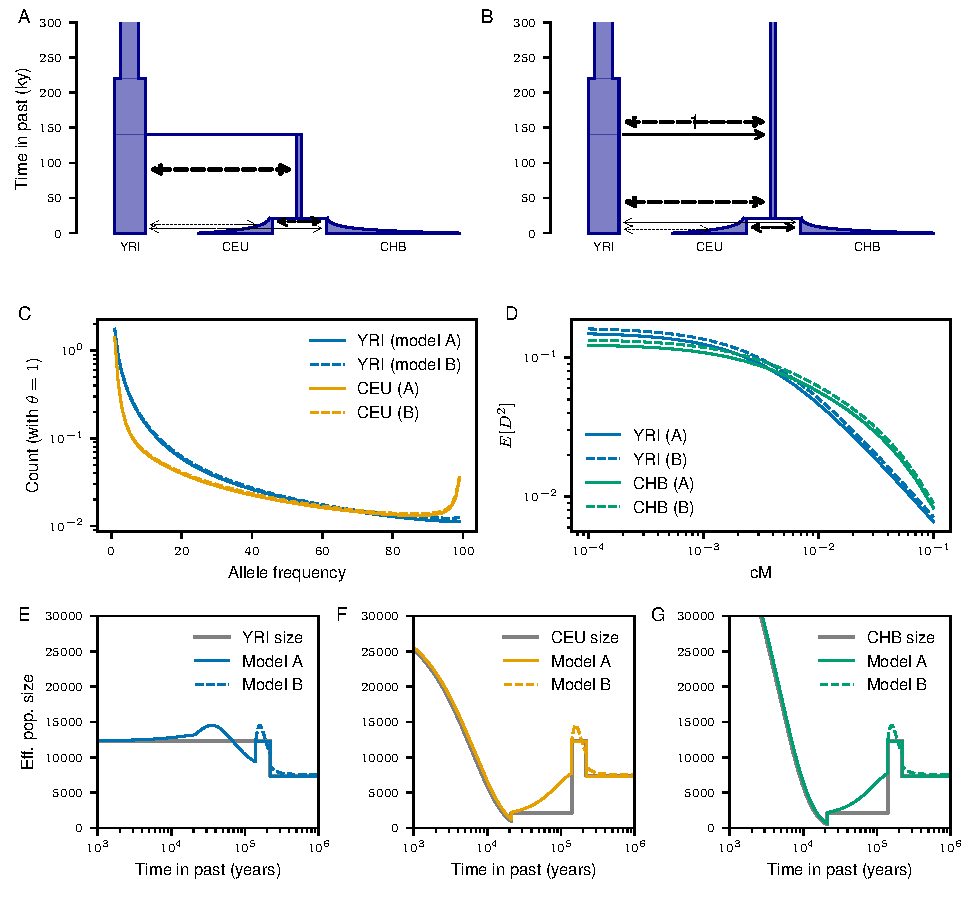
\includegraphics{figures/ooa_expected_stats.pdf}}
\caption{\textbf{Expected diversity statistics under the \citet{gutenkunst2009inferring} model}.
    \textbf{(A)} The correctly implemented model. Dashed arrows depict continuous migration.
    \textbf{(B)} The incorrectly implemented model from the \msprime\ tutorial, with migration continuing
    into the past beyond the mass migration event with proportion $1$ from the ancestral population
    to the bottleneck population.
    \textbf{(C)} Marginal allele frequency spectra under the two models. Heterozygosity in the incorrect model
    is inflated by $\sim3.5\%$, though the general shape of the distributions are qualitatively similar.
    \textbf{(D)} Similarly, the increased heterozygosity leads to excess $D^2$, though the LD-decay is
    qualitatively similar between models.
    \textbf{(E-G)} We compared the true size history for each population under this model to their
    expected inverse coalescent rates, which are often interpreted as $N_e$. The correct and incorrect
    models (A and B) are equivalent in the recent history, so the inverse coalescence rates only differ
    in the more distant past. For multi-population demographic history, the inverse coalescence rates
    are not expected to match the ``true'' historical size along each branch, as population structure and
    migration between populations change coalescent probabilities over time.
}
\label{fig:ooa_stats}
\end{center}
\end{figure}

\begin{figure}[ht]
\begin{center}
\makebox[\textwidth][c]{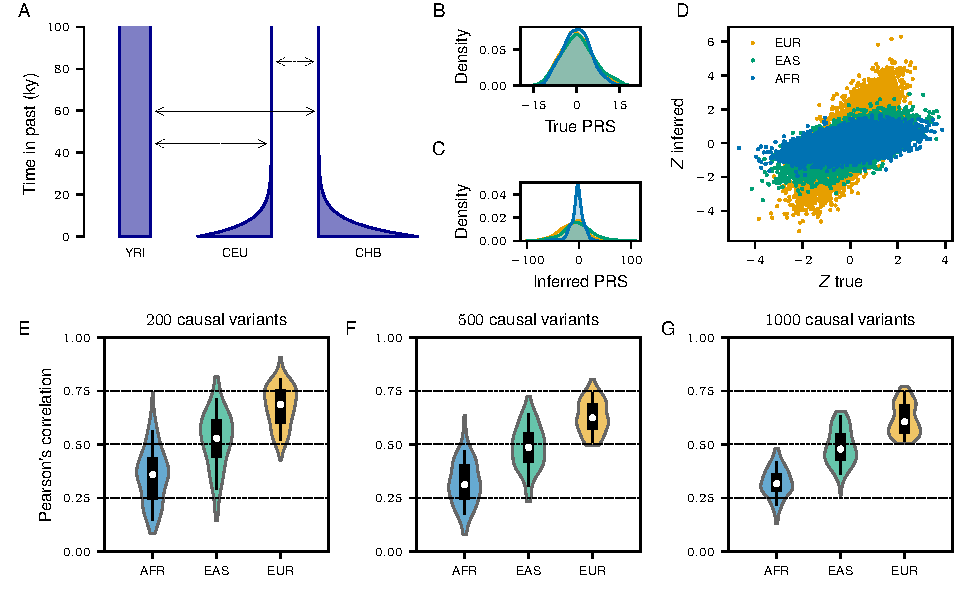
\includegraphics{figures/prs_fig.pdf}}
\caption{\textbf{The transferability of PRS under neutrality}.
    \textbf{(A)} In~\citet{martin2017human}, the simulated demographic model did not apply demographic
    events in the past, so continental populations were simulated as isolated with low levels of migration
    for all time. The correct model has historical events as shown in Fig.~\ref{fig:ooa_stats}A.
    \textbf{(B-G)} We repeated the simulation experiment in~\citet{martin2017human} using the correct
    demographic model.
    GWAS summary statistics were computed from 10,000 case and control subjects in the European
    population, and the distribution of inferred PRS were compared across the three simulated populations.
    Correlations between true and inferred polygenic scores were computed over 100 simulation replicates.
    Unlike the original study, we do not observe large differences in mean inferred PRS across
    the three populations (C, D), and while risk prediction in the African and East Asian populations is
    still reduced compared to the European population, the reduction in prediction accuracy is not as
    large as reported in the original study (E-G).
    Panels B and C show the distribution of true and inferred PRS after standardizing PRS across all individuals
    in the simulation (this is in contrast to Figure 5 in Martin et al., which plotted unstandardized PRS). Because
    the polygenic trait was simulated as a threshold trait, it is the relative distribution of PRS across indivuduals
    that determined cases and controls instead of absolute true or inferred PRS.
    Panel D shows a comparison of PRS distributions for a simulation replicate with 1,000 causal variants.
    For each population in the violin plots, the original correlations from~\citet{martin2017human}
    are shown on the left, and correlations using the correct model are shown on the right.
    For direct comparison to the original study, see Figure~5 in~\citet{martin2017human}.
}
\label{fig:prs}
\end{center}
\end{figure}

\end{document}
